
\documentclass[10pt,a4paper]{article}
\usepackage[margin=22mm]{geometry}
\usepackage{fontspec}
\usepackage{microtype,booktabs,longtable,graphicx,float,amsmath,array,xcolor,pdflscape,enumitem}
\usepackage[font=small,labelfont=bf]{caption}
\usepackage{subcaption}
\usepackage{siunitx}
\sisetup{detect-all}
\usepackage{tikz}
\usetikzlibrary{arrows.meta,positioning,fit,backgrounds}
\usepackage{fancyhdr}
\usepackage[hidelinks]{hyperref}
\definecolor{ssblue}{HTML}{1F5FA8}\definecolor{ssgreen}{HTML}{2A9D4B}\definecolor{ssred}{HTML}{C0392B}
\definecolor{ssorange}{HTML}{E07B1A}
\newcommand{\pass}{\textcolor{ssgreen}{\textbf{PASS}}}
\newcommand{\fail}{\textcolor{ssred}{\textbf{FAIL}}}
\newcommand{\warn}{\textcolor{ssorange}{\textbf{WARN}}}
\pagestyle{fancy}\fancyhf{}
\lhead{\small StyloSynth-555}\rhead{\small Design \& Verification Report}\cfoot{\small\thepage}
\setlength{\headheight}{14pt}
\setlist{nosep,leftmargin=*}

\begin{document}

\begin{titlepage}\centering
\vspace*{25mm}
{\Huge\bfseries StyloSynth-555\par}\vspace{4mm}
{\Large A 555-based stylus synthesizer\par}\vspace{2mm}
{\large Design \& Verification Report\par}\vspace{10mm}
\includegraphics[width=0.85\textwidth]{renders/printed_closeup}\par\vspace{10mm}
{\large 05 October 2026\par}\vspace{2mm}
{\small Design revision v1.2 \quad$\cdot$\quad commit \texttt{ff20aea}\par}
\vfill
\begin{minipage}{0.85\textwidth}\small
\textbf{Abstract.} StyloSynth-555 is a stylophone-style analogue synthesizer with a CMOS 555 oscillator,
a 20-key exposed-copper keyboard, four exact octaves from a binary divider, an LFO vibrato and an LM386
amplifier. It runs on a single 136\,$\times$\,98\,mm two-layer PCB powered from a 9\,V battery. This report
describes the design and presents the automated verification: circuit simulation, a 2000-build
tolerance analysis, schematic/netlist consistency, static electrical-rule checking, power budgets, PCB DRC
and mechanical fit. All 6 verification steps pass. The design has
not yet been validated on hardware.
\end{minipage}
\end{titlepage}
\tableofcontents\newpage

\section{Introduction}
The instrument is inspired by the vintage Stylophone and by the TouchTone555 project. None of the reference
files are reused; this is an independent design that keeps the feature set and fixes the issues the
reference documented:
\begin{itemize}
\item \textbf{Pitch drift with volume} $\rightarrow$ the oscillator gets its own LDO-regulated, RC-filtered
5\,V rail.
\item \textbf{Inexact octaves from capacitor banks} $\rightarrow$ a CD4040 binary divider gives
mathematically exact 2:1 ratios.
\item \textbf{Op-amp unable to drive the speaker} $\rightarrow$ an LM386 power amplifier.
\item \textbf{20 tuning trimmers} $\rightarrow$ fixed 1\,\% resistors plus a two-trimmer (TUNE/SPAN)
calibration, verified statistically in Section~\ref{sec:mc}.
\end{itemize}
The design is fully script-generated. \texttt{circuit.py} is the single source of truth for the
schematic, PCB and BOM, and \texttt{verify\_all.py} re-runs every check in this report.

\section{System architecture}
\begin{figure}[H]\centering
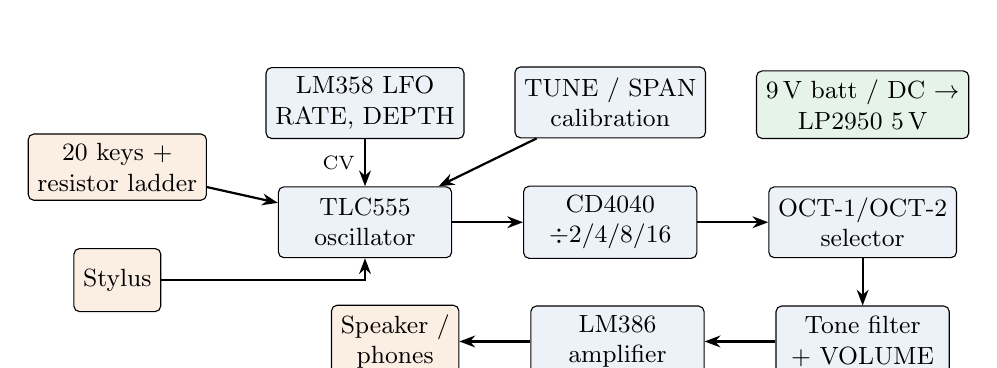
\begin{tikzpicture}[font=\small, node distance=6mm and 9mm,
  blk/.style={draw, rounded corners=2pt, fill=ssblue!8, minimum height=9mm, minimum width=22mm, align=center},
  io/.style={draw, rounded corners=2pt, fill=ssorange!12, minimum height=8mm, align=center},
  pw/.style={draw, rounded corners=2pt, fill=ssgreen!12, minimum height=8mm, align=center},
  ar/.style={-{Stealth[length=2mm]}, thick}]
\node[io] (keys) {20 keys +\\ resistor ladder};
\node[io, below=of keys] (sty) {Stylus};
\node[blk, right=of keys, yshift=-7mm] (osc) {TLC555\\ oscillator};
\node[blk, right=of osc] (div) {CD4040\\ $\div$2/4/8/16};
\node[blk, right=of div] (oct) {OCT-1/OCT-2\\ selector};
\node[blk, below=of oct] (tone) {Tone filter\\ + VOLUME};
\node[blk, left=of tone] (amp) {LM386\\ amplifier};
\node[io, left=of amp] (out) {Speaker /\\ phones};
\node[blk, above=of osc] (lfo) {LM358 LFO\\ RATE, DEPTH};
\node[blk, above=of div] (cal) {TUNE / SPAN\\ calibration};
\node[pw, above=of oct] (pwr) {9\,V batt / DC $\rightarrow$\\ LP2950 5\,V};
\draw[ar] (keys) -- (osc); \draw[ar] (sty) -| (osc);
\draw[ar] (osc) -- (div); \draw[ar] (div) -- (oct); \draw[ar] (oct) -- (tone);
\draw[ar] (tone) -- (amp); \draw[ar] (amp) -- (out);
\draw[ar] (lfo) -- node[left, font=\scriptsize]{CV} (osc); \draw[ar] (cal) -- (osc);
\end{tikzpicture}
\caption{Signal flow. The oscillator, divider and LFO run on a regulated 5\,V rail; the amplifier runs from the raw 9\,V supply.}
\label{fig:block}
\end{figure}

\begin{itemize}
\item \textbf{Oscillator.} A TLC555 in the 50\,\%-duty topology: the output charges the 22\,nF polypropylene
timing capacitor through the key ladder. The stylus picks a tap, so the timing resistance and the pitch depend
on the key touched. A 10\,M$\Omega$ pull-down silences the oscillator when the stylus is lifted.
\item \textbf{Octaves.} The CD4040 divides by 2, 4, 8 or 16. Two DPDT switches form a 2-bit selector.
\item \textbf{Vibrato.} An LM358 relaxation oscillator (3.9--9.6\,Hz) is buffered and AC-coupled through the
DEPTH pot into the 555 control-voltage pin.
\item \textbf{Audio.} A series resistor and switchable tone capacitor feed the VOLUME pot and an LM386 at
gain 20, with a Zobel network and a 220\,$\mu$F output capacitor. The headphone jack's switch contacts
disconnect the speaker and add a 220\,$\Omega$ series resistor.
\item \textbf{Power.} 9\,V battery or 9\,V centre-negative DC (the jack switch disconnects the battery),
Schottky reverse protection, and an LP2950-5.0 LDO behind a 47\,$\Omega$/100\,$\mu$F filter.
\end{itemize}

\section{Circuit design}\subsection{Oscillator and key ladder}
For a rail-to-rail 555 whose thresholds are $V_{CV}$ and $V_{CV}/2$, the capacitor charges towards
$V_{DD}$ and discharges towards 0, so
\begin{equation}
f \;=\; \frac{1}{R\,C_T\left[\ln\dfrac{V_{DD}-V_{CV}/2}{V_{DD}-V_{CV}} + \ln 2\right]},
\qquad R = R_0 + \sum_{i\le k} R_i ,
\end{equation}
where $R_0$ is the 555 output resistance plus the 100\,$\Omega$ stylus resistor. With
$C_T = 22$\,nF and $V_{CV} = 3.296$\,V, the 555 spans
880--2637.02\,Hz. Segment values are chosen greedily from E96 so that
the \emph{cumulative} resistance tracks each target, which means rounding errors never accumulate.

\textbf{Calibration.} TUNE (RV4, 2000\,$\Omega$) adds an offset common to all keys and
is set on key 20. SPAN (RV5, 1000\,$\Omega$) sits in the CV divider: it changes
$V_{CV}$, which scales every frequency by the same factor, and is set on key 1. Two adjustments cancel the
two dominant unknowns ($R_0$ and the $C_T$ tolerance).

\begin{figure}[H]\centering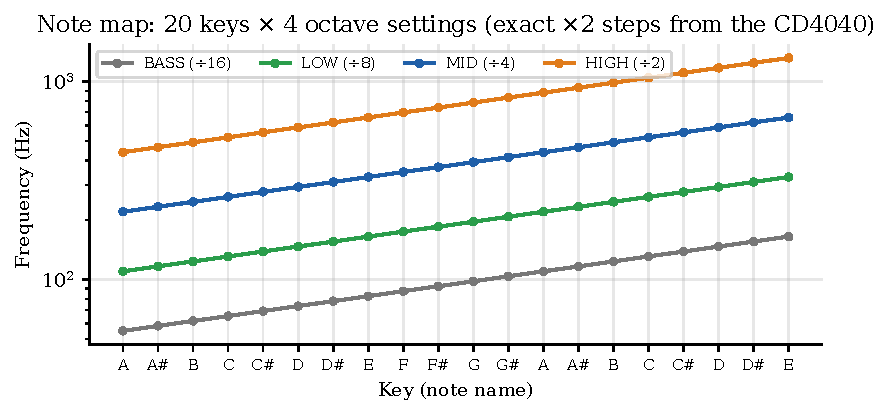
\includegraphics[width=\textwidth]{figures/note_map}\caption{Design frequency of every key at each octave setting.}\label{fig:note_map}\end{figure}

\begin{table}[H]\centering\footnotesize\caption{Ladder values (key 20 is fed first from the 555 output).}\begin{tabular}{rrrrr}\toprule
\textbf{Key} & \textbf{Note (MID)} & \textbf{Segment R ($\Omega$)} & \textbf{$f_{555}$ (Hz)} & \textbf{Output, MID (Hz)} \\ \midrule
1 & A3 & 2k15 & 880.0 & 220.0 \\
2 & A\#3 & 2k & 932.3 & 233.1 \\
3 & B3 & 1k87 & 987.8 & 246.9 \\
4 & C4 & 1k78 & 1046.5 & 261.6 \\
5 & C\#4 & 1k69 & 1108.7 & 277.2 \\
6 & D4 & 1k58 & 1174.7 & 293.7 \\
7 & D\#4 & 1k5 & 1244.5 & 311.1 \\
8 & E4 & 1k4 & 1318.5 & 329.6 \\
9 & F4 & 1k33 & 1396.9 & 349.2 \\
10 & F\#4 & 1k27 & 1480.0 & 370.0 \\
11 & G4 & 1k18 & 1568.0 & 392.0 \\
12 & G\#4 & 1k13 & 1661.2 & 415.3 \\
13 & A4 & 1k05 & 1760.0 & 440.0 \\
14 & A\#4 & 1k & 1864.7 & 466.2 \\
15 & B4 & 953 & 1975.5 & 493.9 \\
16 & C5 & 887 & 2093.0 & 523.2 \\
17 & C\#5 & 845 & 2217.5 & 554.4 \\
18 & D5 & 787 & 2349.3 & 587.3 \\
19 & D\#5 & 750 & 2489.0 & 622.2 \\
20 & E5 & 11k3 + TUNE & 2637.0 & 659.3 \\
\bottomrule\end{tabular}\end{table}

\subsection{Vibrato, audio and power}
The LFO is a single-supply Schmitt relaxation oscillator with $3\times100$\,k$\Omega$ hysteresis and
$R = 68\,\mathrm{k}\Omega + $ RATE (100\,k$\Omega$) into 1\,$\mu$F; its timing node is buffered by the second
op-amp half. A 1.5\,k$\Omega$\,/\,(2.4\,k$\Omega$ + SPAN) external CV divider swamps the TLC555's internal
divider, so the vibrato depth and the calibration don't depend on the 555's internal resistors. In the audio
path, a 150\,k$\Omega$ series resistor sets the LM386 input so full volume just avoids hard clipping at 9\,V.

\section{Simulation results}
All circuit simulations use ngspice (the KiCad 7 shared library) driven from Python. The 555 is modelled
behaviourally as a CV-referenced Schmitt switch with 100\,$\Omega$ output resistance, and the LM358 as a
saturating high-gain stage (0.02--3.5\,V swing at 5\,V).

\begin{figure}[H]\centering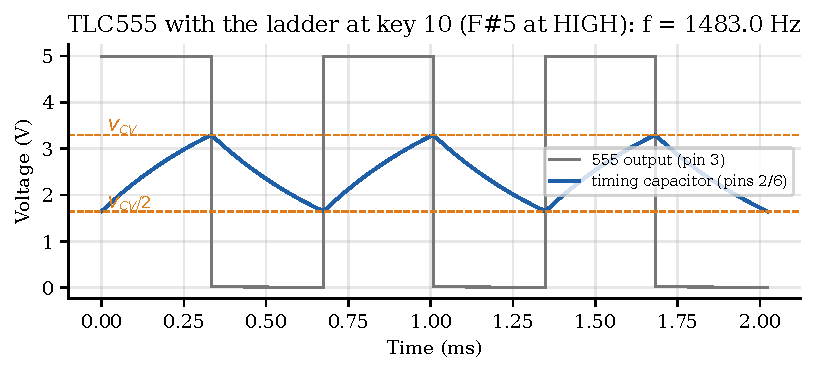
\includegraphics[width=\textwidth]{figures/osc_555}\caption{Oscillator transient: the timing capacitor swings between $V_{CV}/2$ and $V_{CV}$.}\label{fig:osc_555}\end{figure}

\begin{figure}[H]\centering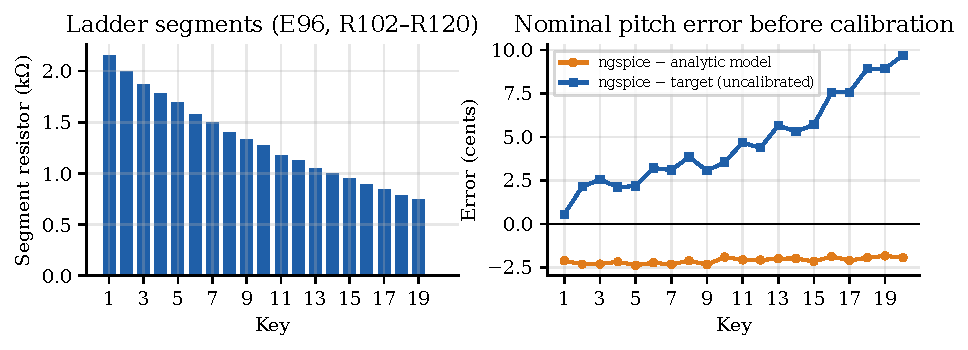
\includegraphics[width=\textwidth]{figures/ladder}\caption{Ladder segment values and nominal (uncalibrated) pitch error. The near-constant offset between simulation and target is removed by TUNE/SPAN; the simulation agrees with the analytic model to within 0.54 cents across all keys.}\label{fig:ladder}\end{figure}

\begin{figure}[H]\centering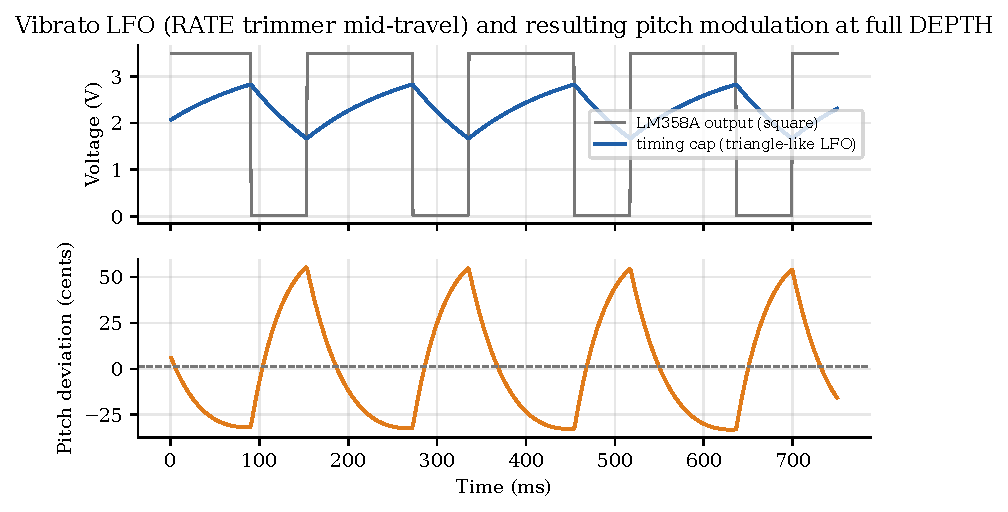
\includegraphics[width=\textwidth]{figures/lfo}\caption{Vibrato LFO waveform and pitch modulation at full DEPTH: -33 to +55 cents. The LM358 output swing is asymmetric (0.02--3.5\,V), so the time-averaged pitch rises by 1 cents while vibrato is on (dashed line). The offset shrinks in proportion to DEPTH; calibration is done with vibrato off.}\label{fig:lfo}\end{figure}

\begin{figure}[H]\centering\begin{subfigure}{0.48\textwidth}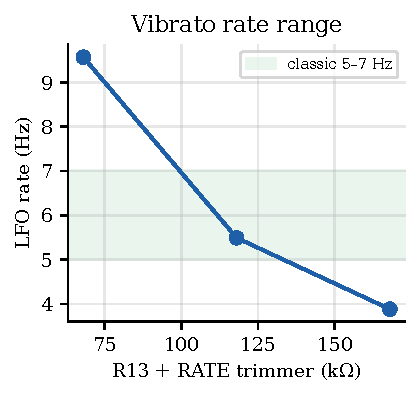
\includegraphics[width=\linewidth]{figures/lfo_rate}\caption{LFO rate vs. RATE setting}\end{subfigure}\hfill\begin{subfigure}{0.5\textwidth}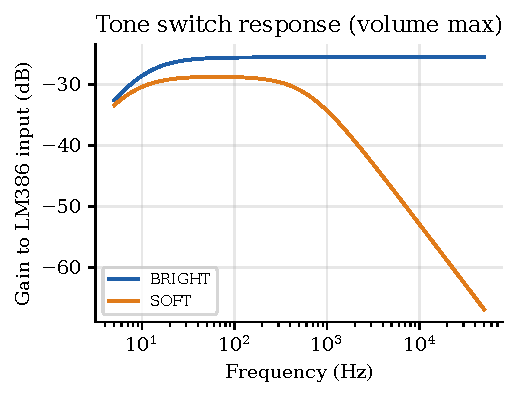
\includegraphics[width=\linewidth]{figures/audio}\caption{Tone response into the LM386}\end{subfigure}\caption{Vibrato rate range and audio path.}\end{figure}
\begin{table}[H]\centering\small\caption{Simulation checks.}\begin{tabular}{llll}\toprule
\textbf{Check} & \textbf{Target} & \textbf{Result} & \textbf{Status} \\ \midrule
Ladder: ngspice vs analytic model & spread < 2 ct & 0.54 ct & \pass \\
LFO rate range & covers 5--7 Hz & 3.88--9.57 Hz & \pass \\
Vibrato depth (full) & 25--80 ct & $\pm$45.6 ct & \pass \\
CV DC with LFO running & 3.296 V & 3.2956 V & \pass \\
LM386 drive, full volume & 2.0--3.8 V pk & 3.35 V pk & \pass \\
Audio HPF corner & < 40 Hz & 10.4 Hz & \pass \\
SOFT LPF corner & 0.5--1 kHz & 629.5 Hz & \pass \\
\bottomrule\end{tabular}\end{table}

\section{Tolerance analysis}\label{sec:mc}
Each simulated build draws random values for: every ladder resistor ($\pm$1\,\% or $\pm$0.1\,\%), $C_T$
($\pm$2.5\,\%), $R_0$ (100--700\,$\Omega$) and the 555 internal divider (20--300\,k$\Omega$). The two-point
calibration is then emulated (TUNE on key 20, SPAN on key 1, iterated) and the error of every key is
measured. The model behind this is the analytic equation, validated against ngspice in the previous section.

\begin{figure}[H]\centering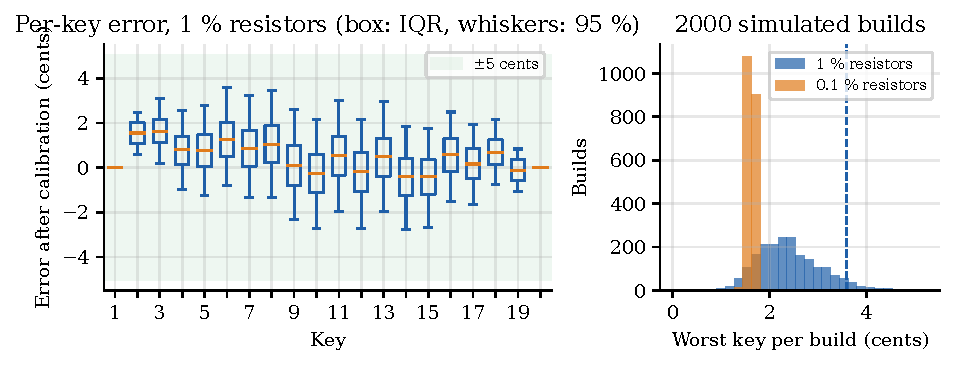
\includegraphics[width=\textwidth]{figures/monte_carlo}\caption{Tuning error after calibration across 2000 simulated builds.}\label{fig:monte_carlo}\end{figure}

\begin{table}[H]\centering\small\caption{Worst-key tuning error per build (1 cent = 1/100 semitone; about 5--10 cents is the threshold of audibility).}\begin{tabular}{lrrrr}\toprule
\textbf{Resistors} & \textbf{Cal. failures} & \textbf{Median worst key} & \textbf{95th pct} & \textbf{Max} \\ \midrule
1 \% (specified) & 0/2000 & 2.34 ct & \textbf{3.59 ct} & 5.01 ct \\
0.1 \% (upgrade) & 0/2000 & 1.62 ct & 1.75 ct & 1.84 ct \\
\bottomrule\end{tabular}\end{table}

\section{Schematic and electrical rules}
The schematic is generated from \texttt{circuit.py} and checked by round-trip: KiCad exports its netlist,
which is compared with the design source. \textbf{Result:} PASS: 59 nets and 81 components match circuit.py.

KiCad~7 has no command-line ERC, so a static rule check runs on the netlist using the official KiCad symbol
pin types. It covers 59 nets and 210 pins, and checks for: multiple drivers on one net,
power inputs without a source, floating inputs and single-pin nets. \textbf{Result: 0
issues} \pass. Waived, intentional cases:
\begin{itemize}\item U2 pin 7 unconnected - TLC555 DIS is an open-drain output (KiCad types it as input); unused in this topology\item U4 pin 1 unconnected - LM386 GAIN pins left open = gain 20 (datasheet default)\item U4 pin 8 unconnected - LM386 GAIN pins left open = gain 20 (datasheet default)\end{itemize}
\begin{figure}[H]\centering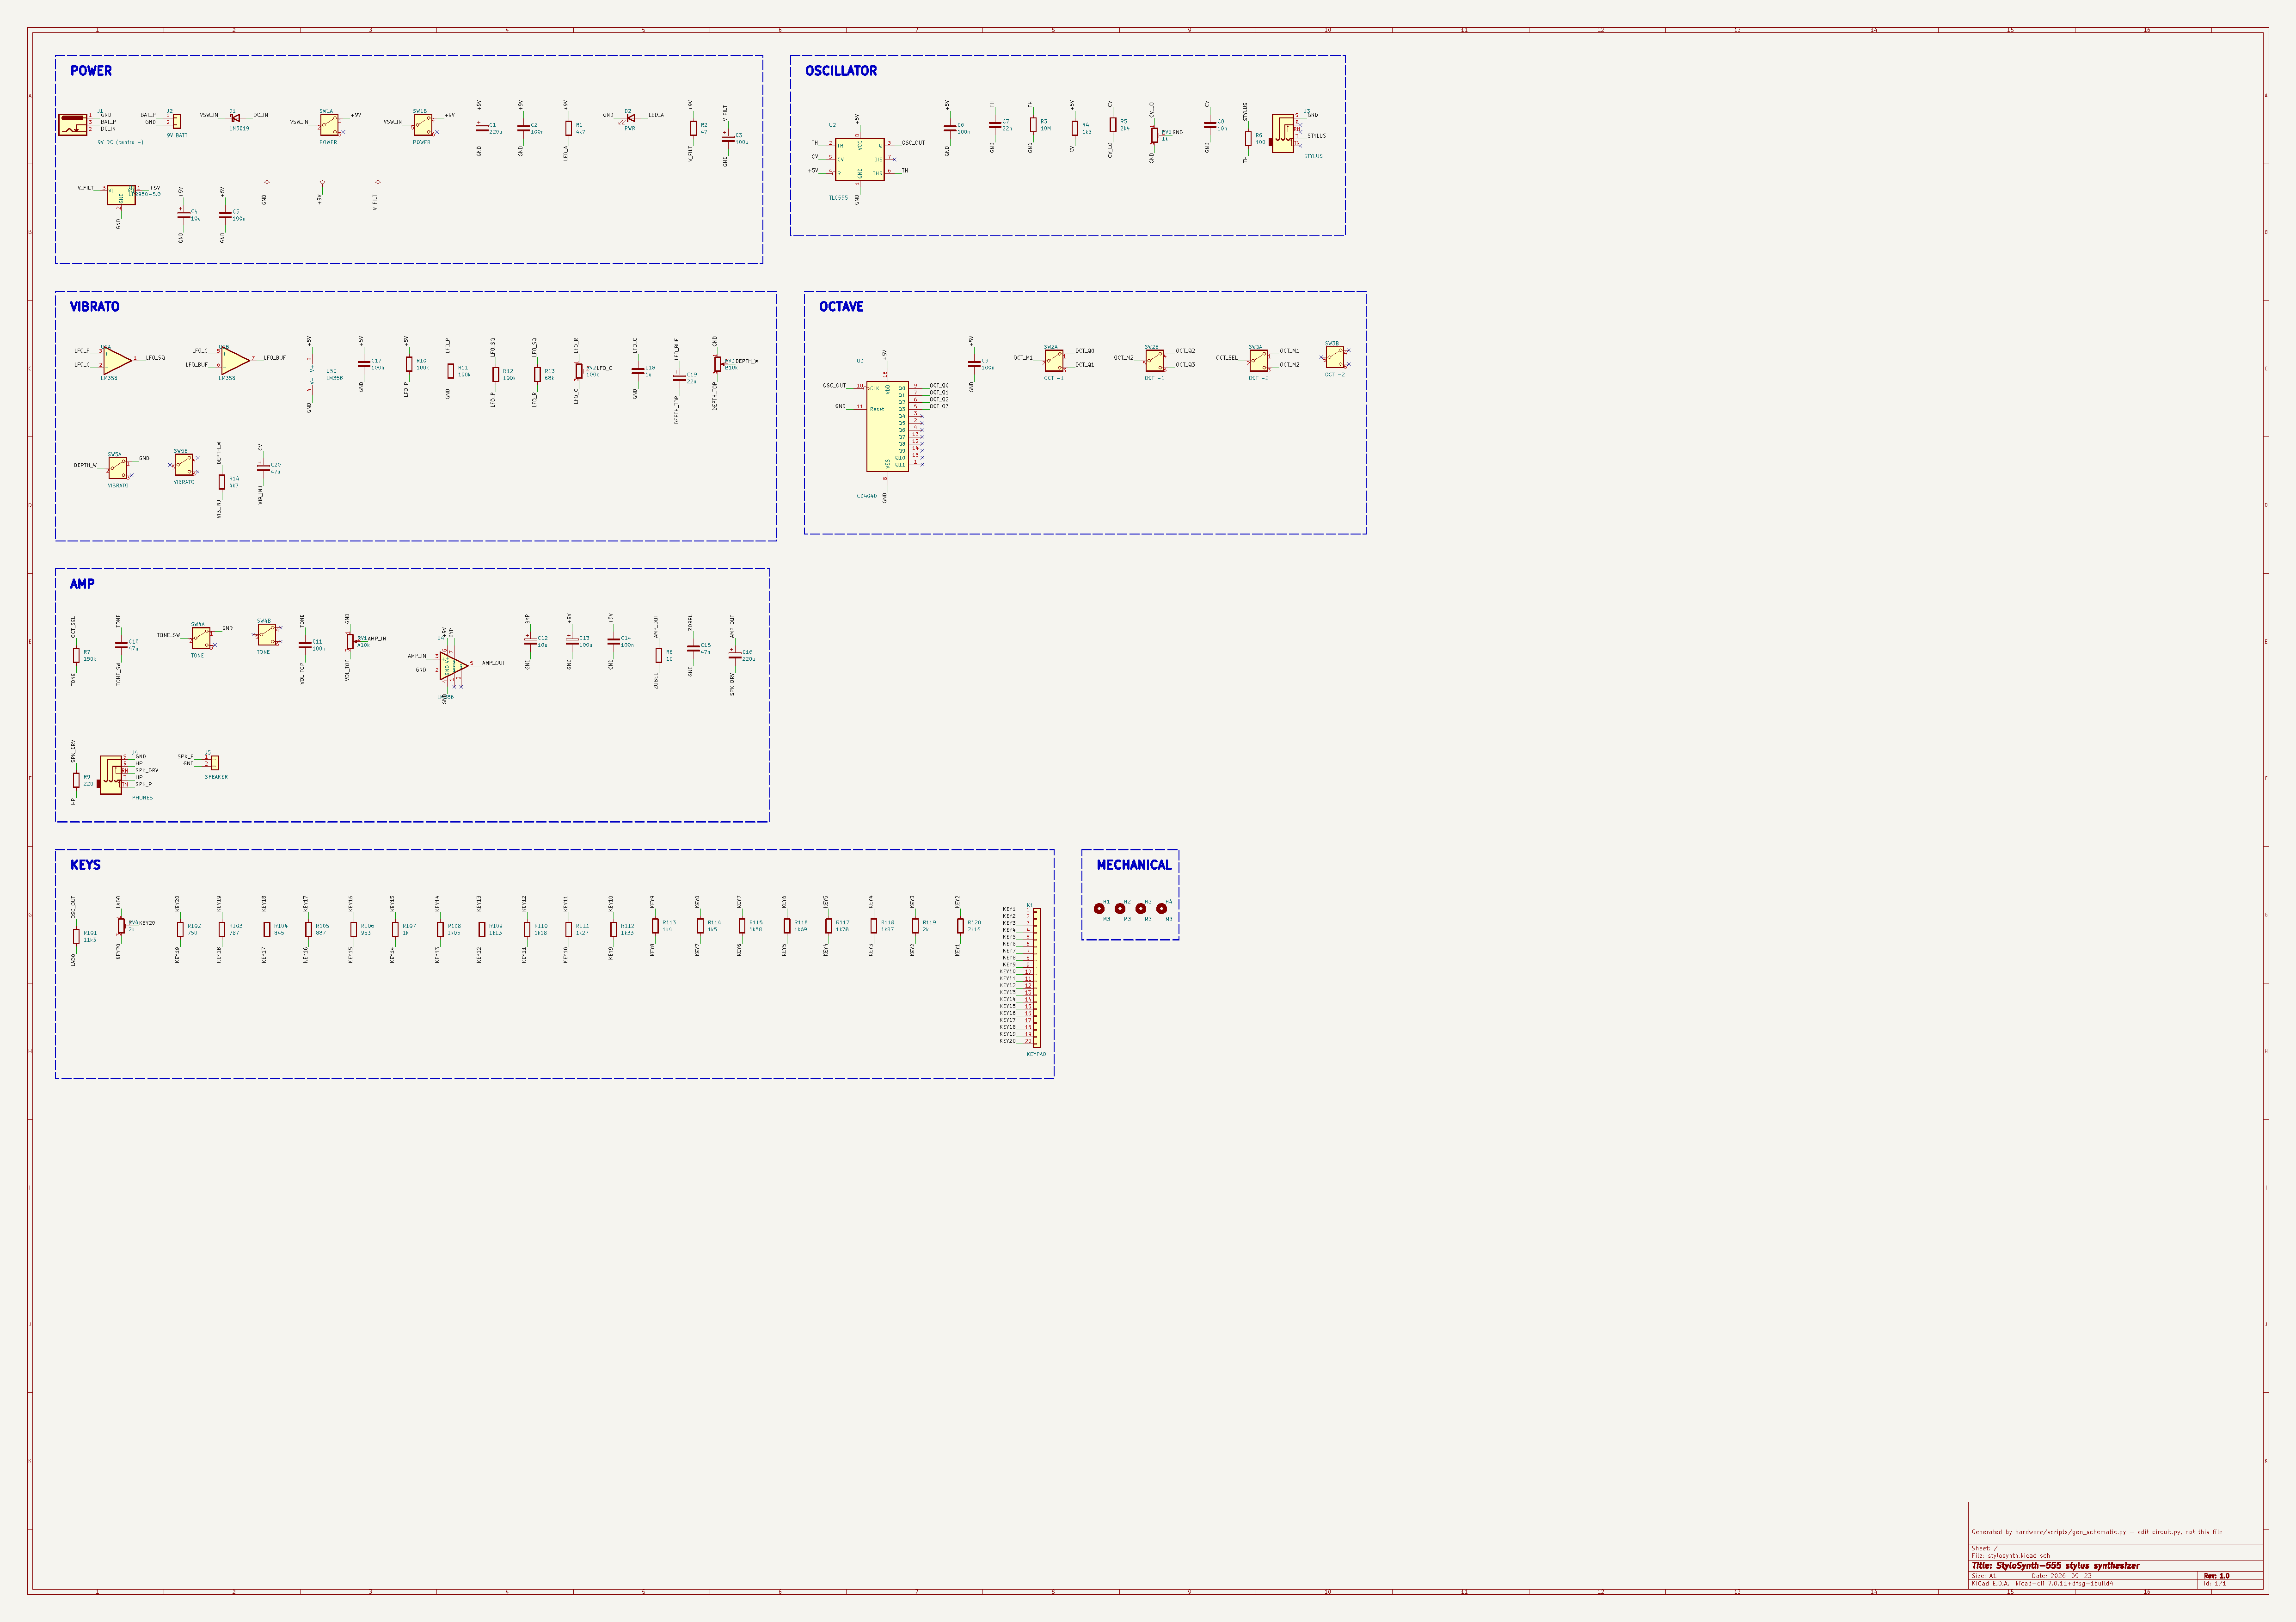
\includegraphics[width=\textwidth]{figures/schematic}
\caption{Generated schematic (vector; the full-size sheet is in Appendix~\ref{app:sch}).}\end{figure}

\section{Power, ratings and dissipation}Datasheet-typical values, not measurements.

\begin{figure}[H]\centering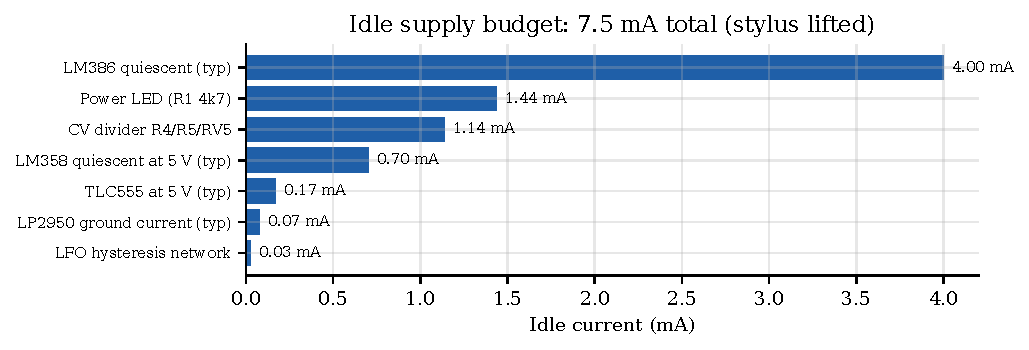
\includegraphics[width=\textwidth]{figures/power}\caption{Idle current budget.}\label{fig:power}\end{figure}

\begin{table}[H]\centering\footnotesize\caption{Power and dissipation checks.}\begin{tabular}{p{5.2cm}p{4.6cm}p{3.4cm}l}\toprule
\textbf{Item} & \textbf{Value} & \textbf{Limit / note} & \textbf{Status} \\ \midrule
Idle supply current & 7.5 mA & $\approx$ 73 h idle on a 550 mAh alkaline 9 V & \pass \\
LM386 output at full volume (sim) & 3.35 V pk $\rightarrow$ 701 mW sine-equivalent into 8 $\Omega$ & use a $\geq$ 1 W speaker & \pass \\
LM386N-1 worst-case dissipation & 549 mW & DIP-8 rating 1.25 W at 25 $^\circ$C & \pass \\
LP2950 dissipation & 10.7 mW at 3 mA & TO-92 rating $\approx$ 600 mW & \pass \\
R9 (220 $\Omega$) with shorted headphone plug & 51 mW & 0.25 W rating & \pass \\
R1 LED resistor & 9.7 mW & 0.25 W rating & \pass \\
D1 1N5819 current / reverse voltage & < 0.3 A / $\leq$ 12 V & 1 A / 40 V rating & \pass \\
\bottomrule\end{tabular}\end{table}

\begin{table}[H]\centering\footnotesize\caption{Capacitor voltage ratings ($\geq$1.25$\times$ the worst-case net voltage; 12\,V assumed on the 9\,V side).}\begin{tabular}{lllll|lllll}\toprule
\textbf{Cap} & \textbf{Value} & \textbf{Rated} & \textbf{Worst} & \textbf{} & \textbf{Cap} & \textbf{Value} & \textbf{Rated} & \textbf{Worst} & \textbf{} \\ \midrule
C1 & 220u & 16 V & 12 V & \pass & C11 & 100n & 63 V & 5 V & \pass \\
C2 & 100n & 50 V & 12 V & \pass & C12 & 10u & 25 V & 12 V & \pass \\
C3 & 100u & 16 V & 12 V & \pass & C13 & 100u & 16 V & 12 V & \pass \\
C4 & 10u & 25 V & 5 V & \pass & C14 & 100n & 50 V & 12 V & \pass \\
C5 & 100n & 50 V & 5 V & \pass & C15 & 47n & 50 V & 5 V & \pass \\
C6 & 100n & 50 V & 5 V & \pass & C16 & 220u & 16 V & 12 V & \pass \\
C7 & 22n & 100 V & 5 V & \pass & C17 & 100n & 50 V & 5 V & \pass \\
C8 & 10n & 50 V & 5 V & \pass & C18 & 1u & 63 V & 5 V & \pass \\
C9 & 100n & 50 V & 5 V & \pass & C19 & 22u & 25 V & 5 V & \pass \\
C10 & 47n & 63 V & 5 V & \pass & C20 & 47u & 25 V & 5 V & \pass \\
\bottomrule\end{tabular}\end{table}

\noindent\textbf{Note:} the LM386N-1 operating range is 4--12\,V, so use a \emph{regulated} 9\,V adapter.

\section{PCB}
136\,$\times$\,98\,mm, two layers, 1.6\,mm FR-4, ENIG finish (the keys are exposed copper). Routed with
Freerouting; the ground net is carried by copper pours on both layers, with the pour kept out of the
keyboard area. Statistics: 81 footprints, 617 track segments, 3 vias,
2/2 pours filled.
\begin{figure}[H]\centering
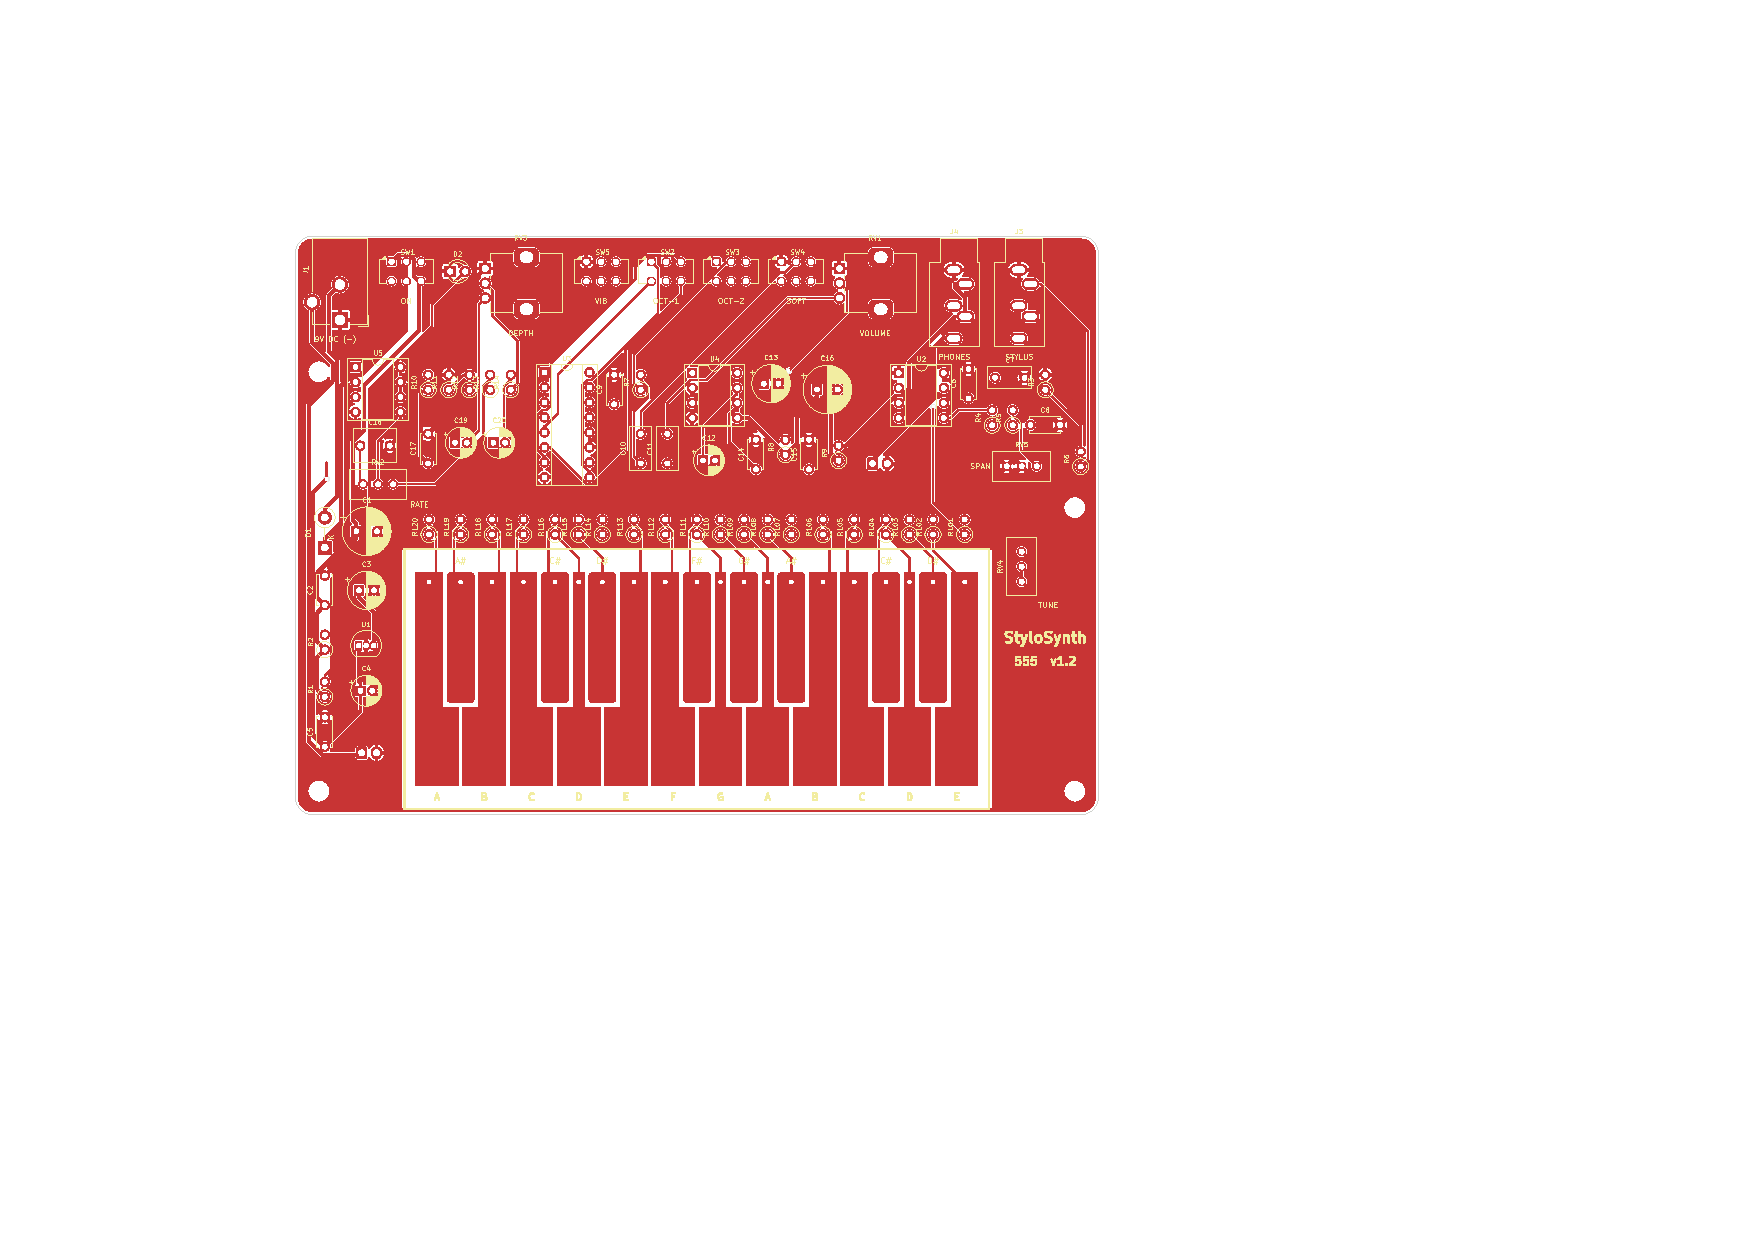
\includegraphics[width=\textwidth, trim=48.0mm 70.0mm 109.0mm 38.0mm, clip]{figures/pcb_front}
\caption{Front copper and silkscreen. The 20 piano-style keys are exposed ENIG pads; the ladder resistors
sit in a row directly above the key vias.}\end{figure}
\begin{figure}[H]\centering
\begin{subfigure}{0.49\textwidth}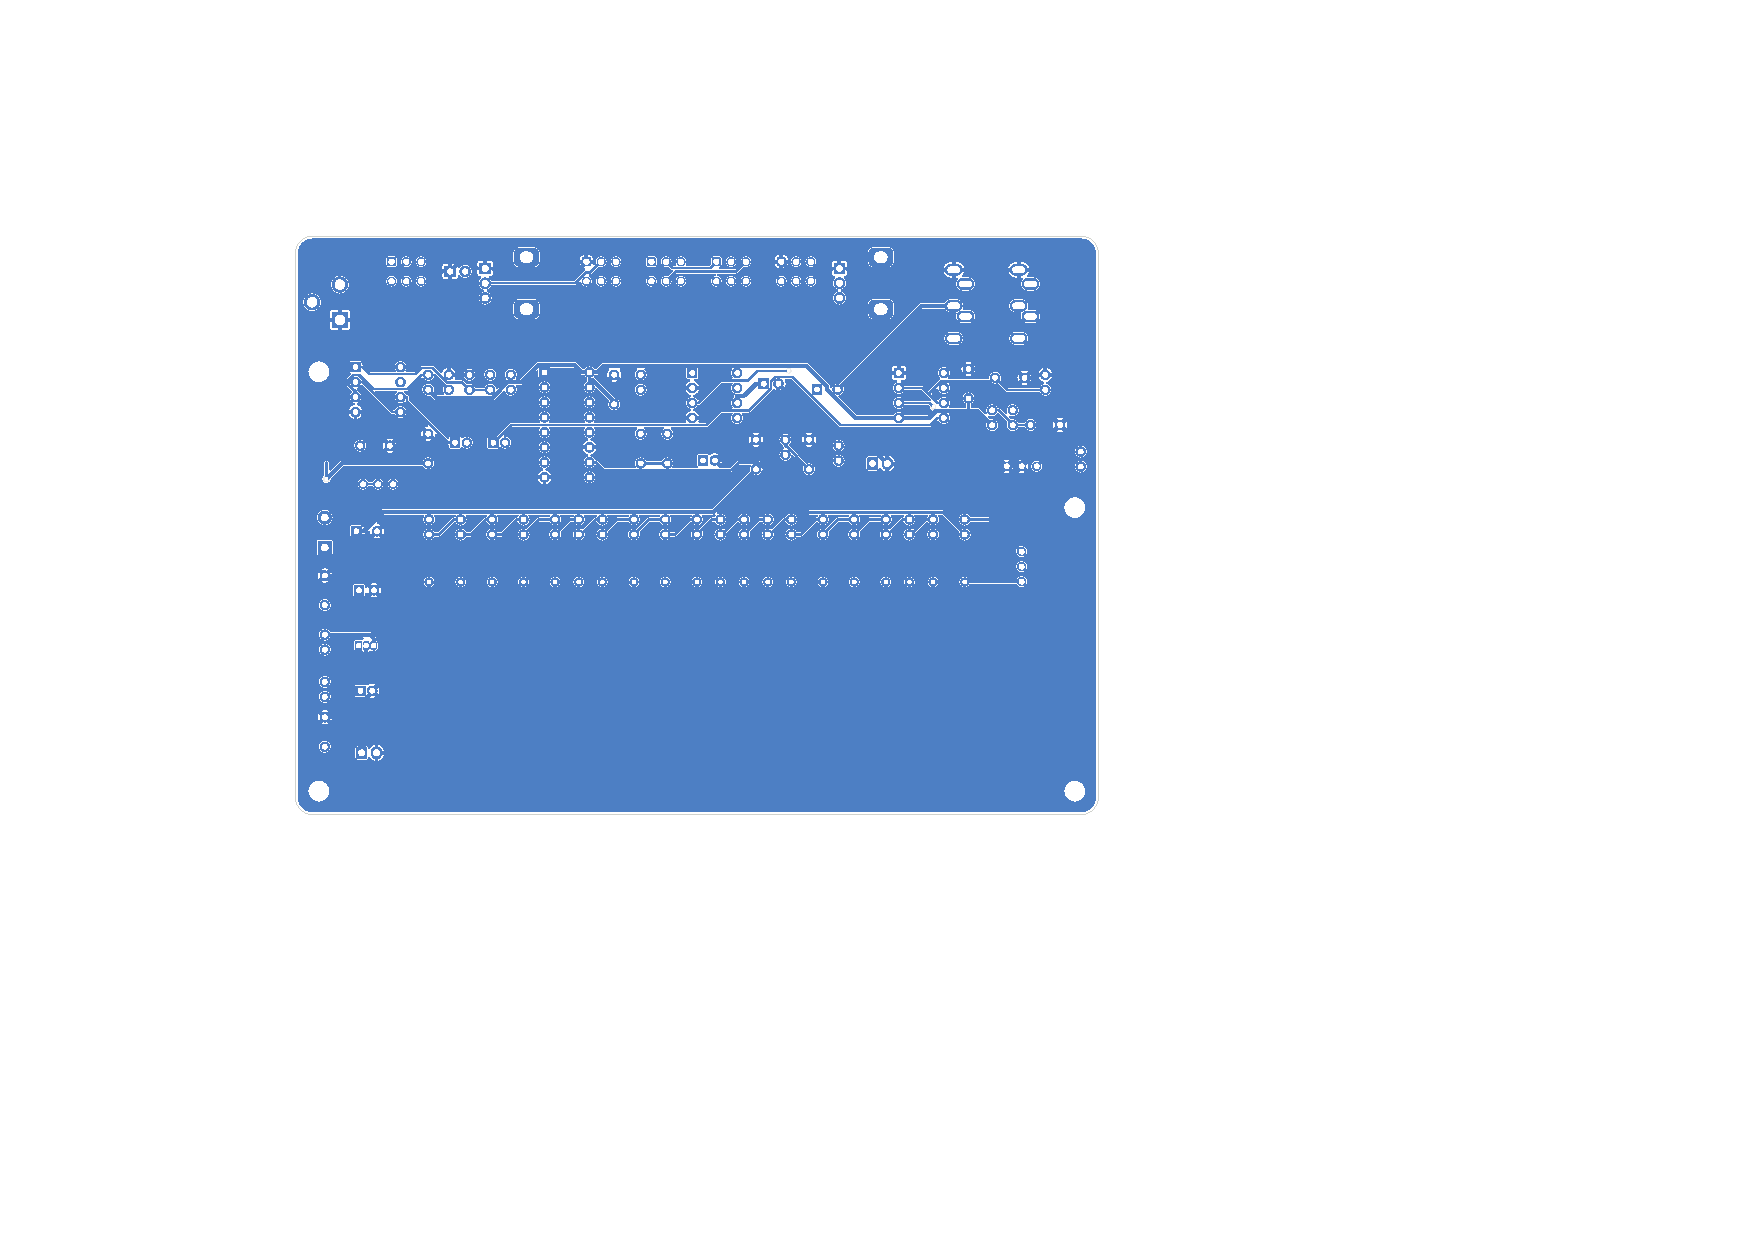
\includegraphics[width=\linewidth, trim=48.0mm 70.0mm 109.0mm 38.0mm, clip]{figures/pcb_back}
\caption{Back copper}\end{subfigure}\hfill
\begin{subfigure}{0.49\textwidth}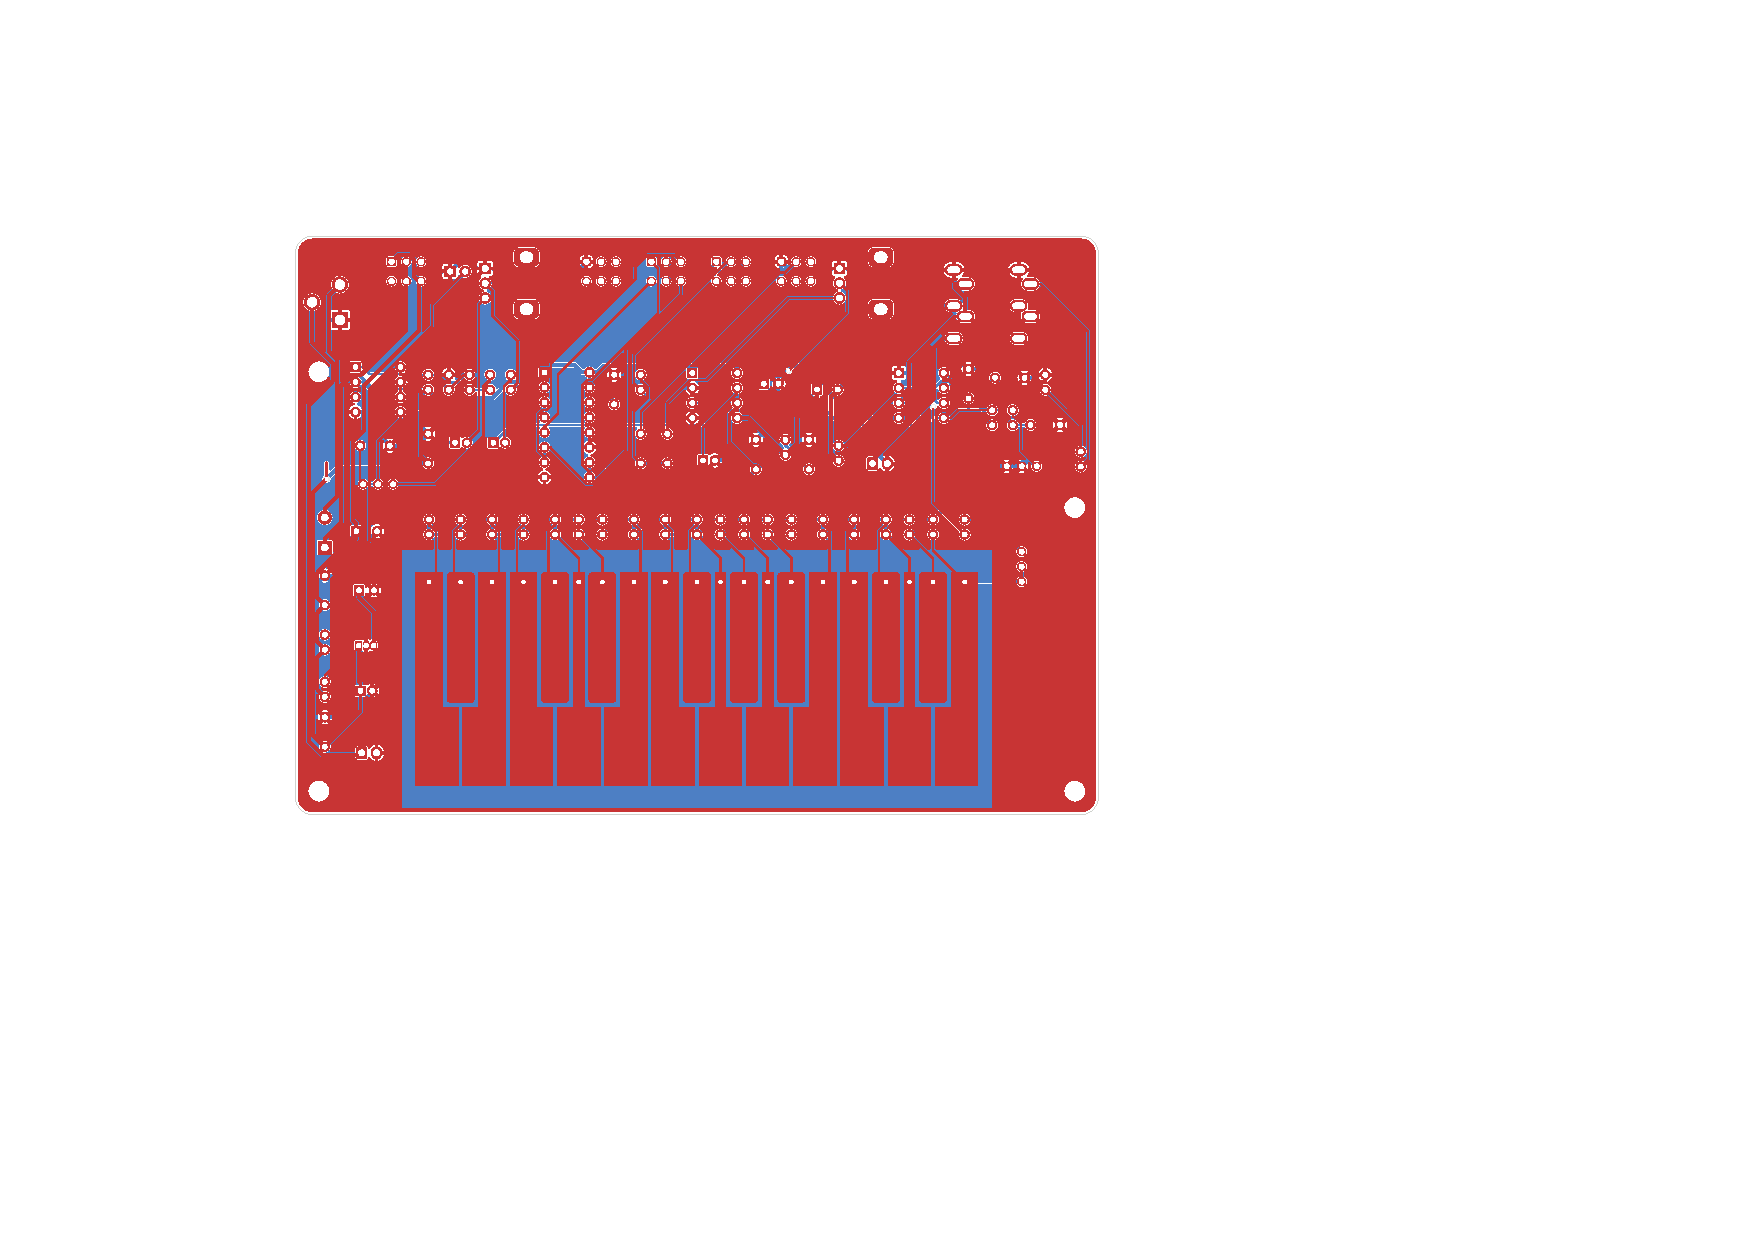
\includegraphics[width=\linewidth, trim=48.0mm 70.0mm 109.0mm 38.0mm, clip]{figures/pcb_copper}
\caption{Both copper layers}\end{subfigure}
\caption{PCB layers.}\end{figure}

\begin{table}[H]\centering\footnotesize\caption{PCB verification.}\begin{tabular}{p{6cm}p{6.2cm}l}\toprule
\textbf{Check} & \textbf{Result} & \textbf{Status} \\ \midrule
DRC errors (incl. unconnected items) & 0 & \pass \\
DRC warnings (cosmetic) & silk\_overlap 23, silk\_over\_copper 5, silk\_edge\_clearance 2, track\_dangling 2 & -- \\
Schematic $\leftrightarrow$ PCB pad nets & 0 mismatches / 210 pins & \pass \\
Min. track width & Default 0.25 mm, Ground 0.50 mm, Power 0.50 mm & -- \\
Decoupling U2 pin 8 (+5V) & C6 (100n) at 6.0 mm & \pass \\
Decoupling U3 pin 16 (+5V) & C9 (100n) at 6.8 mm & \pass \\
Decoupling U4 pin 6 (+9V) & C13 (100u) at 5.6 mm & \pass \\
Decoupling U5 pin 8 (+5V) & C17 (100n) at 17.0 mm & \warn \\
Decoupling U1 pin 1 (+5V) & C4 (10u) at 7.6 mm & \pass \\
\bottomrule\end{tabular}\end{table}

\noindent\textbf{Finding:} U5 pin 8 (+5V): nearest decoupling cap C17 is 17.0 mm away (target < 12 mm). Move C17 next to the supply pin in the next revision. Severity is low: U5 only runs the vibrato LFO, from the LDO-filtered rail.

\section{Enclosures}
Both enclosures use the PCB as the top face, held at its four M3 holes. The battery and speaker sit
underneath, and all jacks and switches stand above the enclosure edge, so no cut-outs are needed. A geometric
fit check confirms the battery, speaker, bosses and pillars clear the back-side parts and THT leads by at
least 1\,mm. \textbf{Result:} fit check: PASS (battery, speaker, bosses, pillars clear of back-side parts and leads).
\begin{figure}[H]\centering\includegraphics[width=\textwidth]{renders/enclosures_overview}
\caption{3D-printed tray with stylus (left) and laser-cut acrylic stack (right), modelled in Blender with
the textured PCB and components.}\end{figure}
\begin{figure}[H]\centering
\begin{subfigure}{0.49\textwidth}\includegraphics[width=\linewidth]{renders/printed_closeup}
\caption{Printed tray: PETG, 141.8$\times$103.8$\times$25.6\,mm, $\approx$62\,cm$^3$}\end{subfigure}\hfill
\begin{subfigure}{0.49\textwidth}\includegraphics[width=\linewidth]{renders/acrylic_closeup}
\caption{Acrylic: 1 base + 8 rings, 3\,mm, 151$\times$113\,mm}\end{subfigure}
\caption{Enclosure variants.}\end{figure}

\section{Verification summary}\begin{table}[H]\centering\small\caption{Automated verification.}\begin{tabular}{clp{5.2cm}l}\toprule
\textbf{\#} & \textbf{Check} & \textbf{Method} & \textbf{Result} \\ \midrule
1 & Circuit behaviour & ngspice, behavioural models & \pass \\
2 & Tuning accuracy & 2000-build tolerance analysis + calibration & \pass \\
3 & Schematic vs source & netlist round-trip & \pass \\
4 & Electrical rules & static ERC on symbol pin types & \pass \\
5 & Power and ratings & hand calculations & \pass \\
6 & PCB & DRC, parity, decoupling & \pass \\
7 & Mechanical fit & geometry check & \pass \\
\bottomrule\end{tabular}\end{table}


\subsection*{Not yet verified}
\begin{itemize}
\item Jack and switch pin behaviour (SJ1-3535NG speaker mute, PJ-102AH battery break, JS202011 slider sense),
assumed from KiCad symbols. Check against the datasheets and on a breadboard.
\item Real IC behaviour with vendor SPICE models (TLC555 output resistance, LM386 stability and hum).
\item KiCad GUI ERC (Inspect $\rightarrow$ Electrical Rules Checker).
\item Physical footprint fit: print the PCB at 1:1 and test-fit the pots, switches, jacks and trimmers.
\item Stylus-lift clicks, ESD, finger hum, and 5\,V rail ripple at full volume, on a prototype.
\end{itemize}

\appendix\section{Bill of materials}{\scriptsize\begin{longtable}{rp{3.6cm}lp{2.2cm}p{4.6cm}r}\caption{BOM (estimated prices, total \$66.22). Full detail in \texttt{bom/bom.csv}.}\\\toprule
\textbf{Qty} & \textbf{Refs} & \textbf{Value} & \textbf{Mfr} & \textbf{MPN / description} & \textbf{USD} \\ \midrule\endfirsthead
\toprule \textbf{Qty} & \textbf{Refs} & \textbf{Value} & \textbf{Mfr} & \textbf{MPN / description} & \textbf{USD} \\ \midrule\endhead
2 & C1, C16 & 220u & Panasonic & EEU-FC1C221 (220uF 16V, 8 mm, 3.5 mm pitch) & 0.90 \\
6 & C2, C5, C6, C9, C14, C17 & 100n & KEMET & C322C104K5R5TA & 1.50 \\
2 & C3, C13 & 100u & Panasonic & EEU-FC1C101 (100uF 16V, 6.3 mm, 2.5 mm pitch) & 0.70 \\
2 & C4, C12 & 10u & Panasonic & EEU-FC1E100 (10uF 25V, 5 mm, 2 mm pitch) & 0.50 \\
1 & C7 & 22n & WIMA & MKP2 22nF 100V 2.5\% 5 mm (polypropylene) & 0.60 \\
1 & C8 & 10n & KEMET & C322C103K5R5TA & 0.25 \\
1 & C10 & 47n & WIMA & MKS2 47nF 63V 5 mm & 0.35 \\
1 & C11 & 100n & WIMA & MKS2 100nF 63V 5 mm & 0.35 \\
1 & C15 & 47n & KEMET & C322C473K5R5TA & 0.25 \\
1 & C18 & 1u & WIMA & MKS2 1uF 63V 5 mm & 0.60 \\
1 & C19 & 22u & Panasonic & EEU-FC1E220 (22uF 25V, 5 mm, 2 mm pitch) & 0.30 \\
1 & C20 & 47u & Panasonic & 47uF 16V, 5 mm dia, 2 mm pitch (FC/FR series) & 0.30 \\
1 & D1 & 1N5819 & onsemi / Vishay & 1N5819 & 0.20 \\
1 & D2 & PWR & Kingbright & WP710A10ID (3 mm red diffused) & 0.25 \\
1 & J1 & 9V DC (centre -) & Same Sky (CUI) & PJ-102AH (5.5x2.1 mm) & 0.90 \\
1 & J2 & 9V BATT & JST & B2B-XH-A(LF)(SN) & 0.15 \\
1 & J3 & STYLUS & Same Sky (CUI) & SJ1-3535NG & 1.30 \\
1 & J4 & PHONES & Same Sky (CUI) & SJ1-3535NG & 1.30 \\
1 & J5 & SPEAKER & JST & B2B-XH-A(LF)(SN) & 0.15 \\
2 & R1, R14 & 4k7 & Yageo / generic & 4k7 metal film 1\% 0.25 W (e.g. Yageo MFR-25\ldots{} & 0.06 \\
1 & R2 & 47 & Yageo / generic & 47 metal film 1\% 0.25 W (e.g. Yageo MFR-25 \ldots{} & 0.03 \\
1 & R3 & 10M & Yageo / generic & 10M metal film 1\% 0.25 W (e.g. Yageo MFR-25\ldots{} & 0.03 \\
2 & R4, R114 & 1k5 & Yageo / generic & 1k5 metal film 1\% 0.25 W (e.g. Yageo MFR-25\ldots{} & 0.06 \\
1 & R5 & 2k4 & Yageo / generic & 2k4 metal film 1\% 0.25 W (e.g. Yageo MFR-25\ldots{} & 0.03 \\
1 & R6 & 100 & Yageo / generic & 100 metal film 1\% 0.25 W (e.g. Yageo MFR-25\ldots{} & 0.03 \\
1 & R7 & 150k & Yageo / generic & 150k metal film 1\% 0.25 W (e.g. Yageo MFR-2\ldots{} & 0.03 \\
1 & R8 & 10 & Yageo / generic & 10 metal film 1\% 0.25 W (e.g. Yageo MFR-25 \ldots{} & 0.03 \\
1 & R9 & 220 & Yageo / generic & 220 metal film 1\% 0.25 W (e.g. Yageo MFR-25\ldots{} & 0.03 \\
3 & R10, R11, R12 & 100k & Yageo / generic & 100k metal film 1\% 0.25 W (e.g. Yageo MFR-2\ldots{} & 0.09 \\
1 & R13 & 68k & Yageo / generic & 68k metal film 1\% 0.25 W (e.g. Yageo MFR-25\ldots{} & 0.03 \\
1 & R101 & 11k3 & Yageo / generic & 11k3 metal film 1\% 0.25 W (e.g. Yageo MFR-2\ldots{} & 0.03 \\
1 & R102 & 750 & Yageo / generic & 750 metal film 1\% 0.25 W (e.g. Yageo MFR-25\ldots{} & 0.03 \\
1 & R103 & 787 & Yageo / generic & 787 metal film 1\% 0.25 W (e.g. Yageo MFR-25\ldots{} & 0.03 \\
1 & R104 & 845 & Yageo / generic & 845 metal film 1\% 0.25 W (e.g. Yageo MFR-25\ldots{} & 0.03 \\
1 & R105 & 887 & Yageo / generic & 887 metal film 1\% 0.25 W (e.g. Yageo MFR-25\ldots{} & 0.03 \\
1 & R106 & 953 & Yageo / generic & 953 metal film 1\% 0.25 W (e.g. Yageo MFR-25\ldots{} & 0.03 \\
1 & R107 & 1k & Yageo / generic & 1k metal film 1\% 0.25 W (e.g. Yageo MFR-25 \ldots{} & 0.03 \\
1 & R108 & 1k05 & Yageo / generic & 1k05 metal film 1\% 0.25 W (e.g. Yageo MFR-2\ldots{} & 0.03 \\
1 & R109 & 1k13 & Yageo / generic & 1k13 metal film 1\% 0.25 W (e.g. Yageo MFR-2\ldots{} & 0.03 \\
1 & R110 & 1k18 & Yageo / generic & 1k18 metal film 1\% 0.25 W (e.g. Yageo MFR-2\ldots{} & 0.03 \\
1 & R111 & 1k27 & Yageo / generic & 1k27 metal film 1\% 0.25 W (e.g. Yageo MFR-2\ldots{} & 0.03 \\
1 & R112 & 1k33 & Yageo / generic & 1k33 metal film 1\% 0.25 W (e.g. Yageo MFR-2\ldots{} & 0.03 \\
1 & R113 & 1k4 & Yageo / generic & 1k4 metal film 1\% 0.25 W (e.g. Yageo MFR-25\ldots{} & 0.03 \\
1 & R115 & 1k58 & Yageo / generic & 1k58 metal film 1\% 0.25 W (e.g. Yageo MFR-2\ldots{} & 0.03 \\
1 & R116 & 1k69 & Yageo / generic & 1k69 metal film 1\% 0.25 W (e.g. Yageo MFR-2\ldots{} & 0.03 \\
1 & R117 & 1k78 & Yageo / generic & 1k78 metal film 1\% 0.25 W (e.g. Yageo MFR-2\ldots{} & 0.03 \\
1 & R118 & 1k87 & Yageo / generic & 1k87 metal film 1\% 0.25 W (e.g. Yageo MFR-2\ldots{} & 0.03 \\
1 & R119 & 2k & Yageo / generic & 2k metal film 1\% 0.25 W (e.g. Yageo MFR-25 \ldots{} & 0.03 \\
1 & R120 & 2k15 & Yageo / generic & 2k15 metal film 1\% 0.25 W (e.g. Yageo MFR-2\ldots{} & 0.03 \\
1 & RV1 & A10k & Alps Alpine / generic & RK09K series 9 mm vertical, 10k log (A10K),\ldots{} & 1.50 \\
1 & RV2 & 100k & Bourns & 3296W-1-104LF & 1.60 \\
1 & RV3 & B10k & Alps Alpine / generic & RK09K series 9 mm vertical, 10k lin (B10K),\ldots{} & 1.50 \\
1 & RV4 & 2k & Bourns & 3296W-1-202LF & 1.60 \\
1 & RV5 & 1k & Bourns & 3296W-1-102LF & 1.60 \\
1 & SW1 & POWER & C\&K & JS202011CQN & 0.60 \\
1 & SW2 & OCT -1 & C\&K & JS202011CQN & 0.60 \\
1 & SW3 & OCT -2 & C\&K & JS202011CQN & 0.60 \\
1 & SW4 & TONE & C\&K & JS202011CQN & 0.60 \\
1 & SW5 & VIBRATO & C\&K & JS202011CQN & 0.60 \\
1 & U1 & LP2950-5.0 & Texas Instruments & LP2950ACZ-5.0/NOPB & 1.00 \\
1 & U2 & TLC555 & Texas Instruments & TLC555CP & 1.10 \\
1 & U3 & CD4040 & Texas Instruments & CD4040BE & 0.70 \\
1 & U4 & LM386 & Texas Instruments & LM386N-1/NOPB & 1.20 \\
1 & U5 & LM358 & Texas Instruments & LM358P & 0.45 \\
3 & - & - & generic & DIP-8 machined socket & 0.90 \\
1 & - & - & generic & DIP-16 machined socket & 0.40 \\
1 & - & - & generic & 8R 1W 40 mm & 2.50 \\
1 & - & - & generic & 9V snap, 150 mm leads & 0.40 \\
4 & - & - & JST & XHP-2 + SXH-001T-P0.6 & 0.80 \\
1 & - & - & generic & 3.5 mm mono plug + cable & 2.00 \\
1 & - & - & generic & brass tip & 0.50 \\
2 & - & - & generic & 6 mm knob & 1.60 \\
4 & - & - & generic & Ruthex-style M3x5.7 & 0.60 \\
4 & - & - & generic & ISO 7380 M3x6 & 0.20 \\
4 & - & - & generic & M3x25 F-F standoff & 1.00 \\
8 & - & - & generic & ISO 7380 M3x6 & 0.40 \\
4 & - & - & generic & ISO 7380 M3x30 + DIN 934 & 0.40 \\
1 & - & - & Ponoko/local laser & see enclosure/out/acrylic/*.dxf & 15.00 \\
4 & - & - & generic & 10 mm bumpon & 0.40 \\
1 & - & - & JLCPCB/PCBWay & fab order & 12.00 \\
\bottomrule\end{longtable}}

\section{Schematic}\label{app:sch}
The complete generated schematic follows on the next page (landscape, vector: zoom in for detail). The source
file is \texttt{hardware/kicad/stylosynth.kicad\_sch}.
\newpage\newgeometry{margin=8mm}\thispagestyle{empty}
\special{pdf:put @thispage << /Rotate 90 >>}
\begin{center}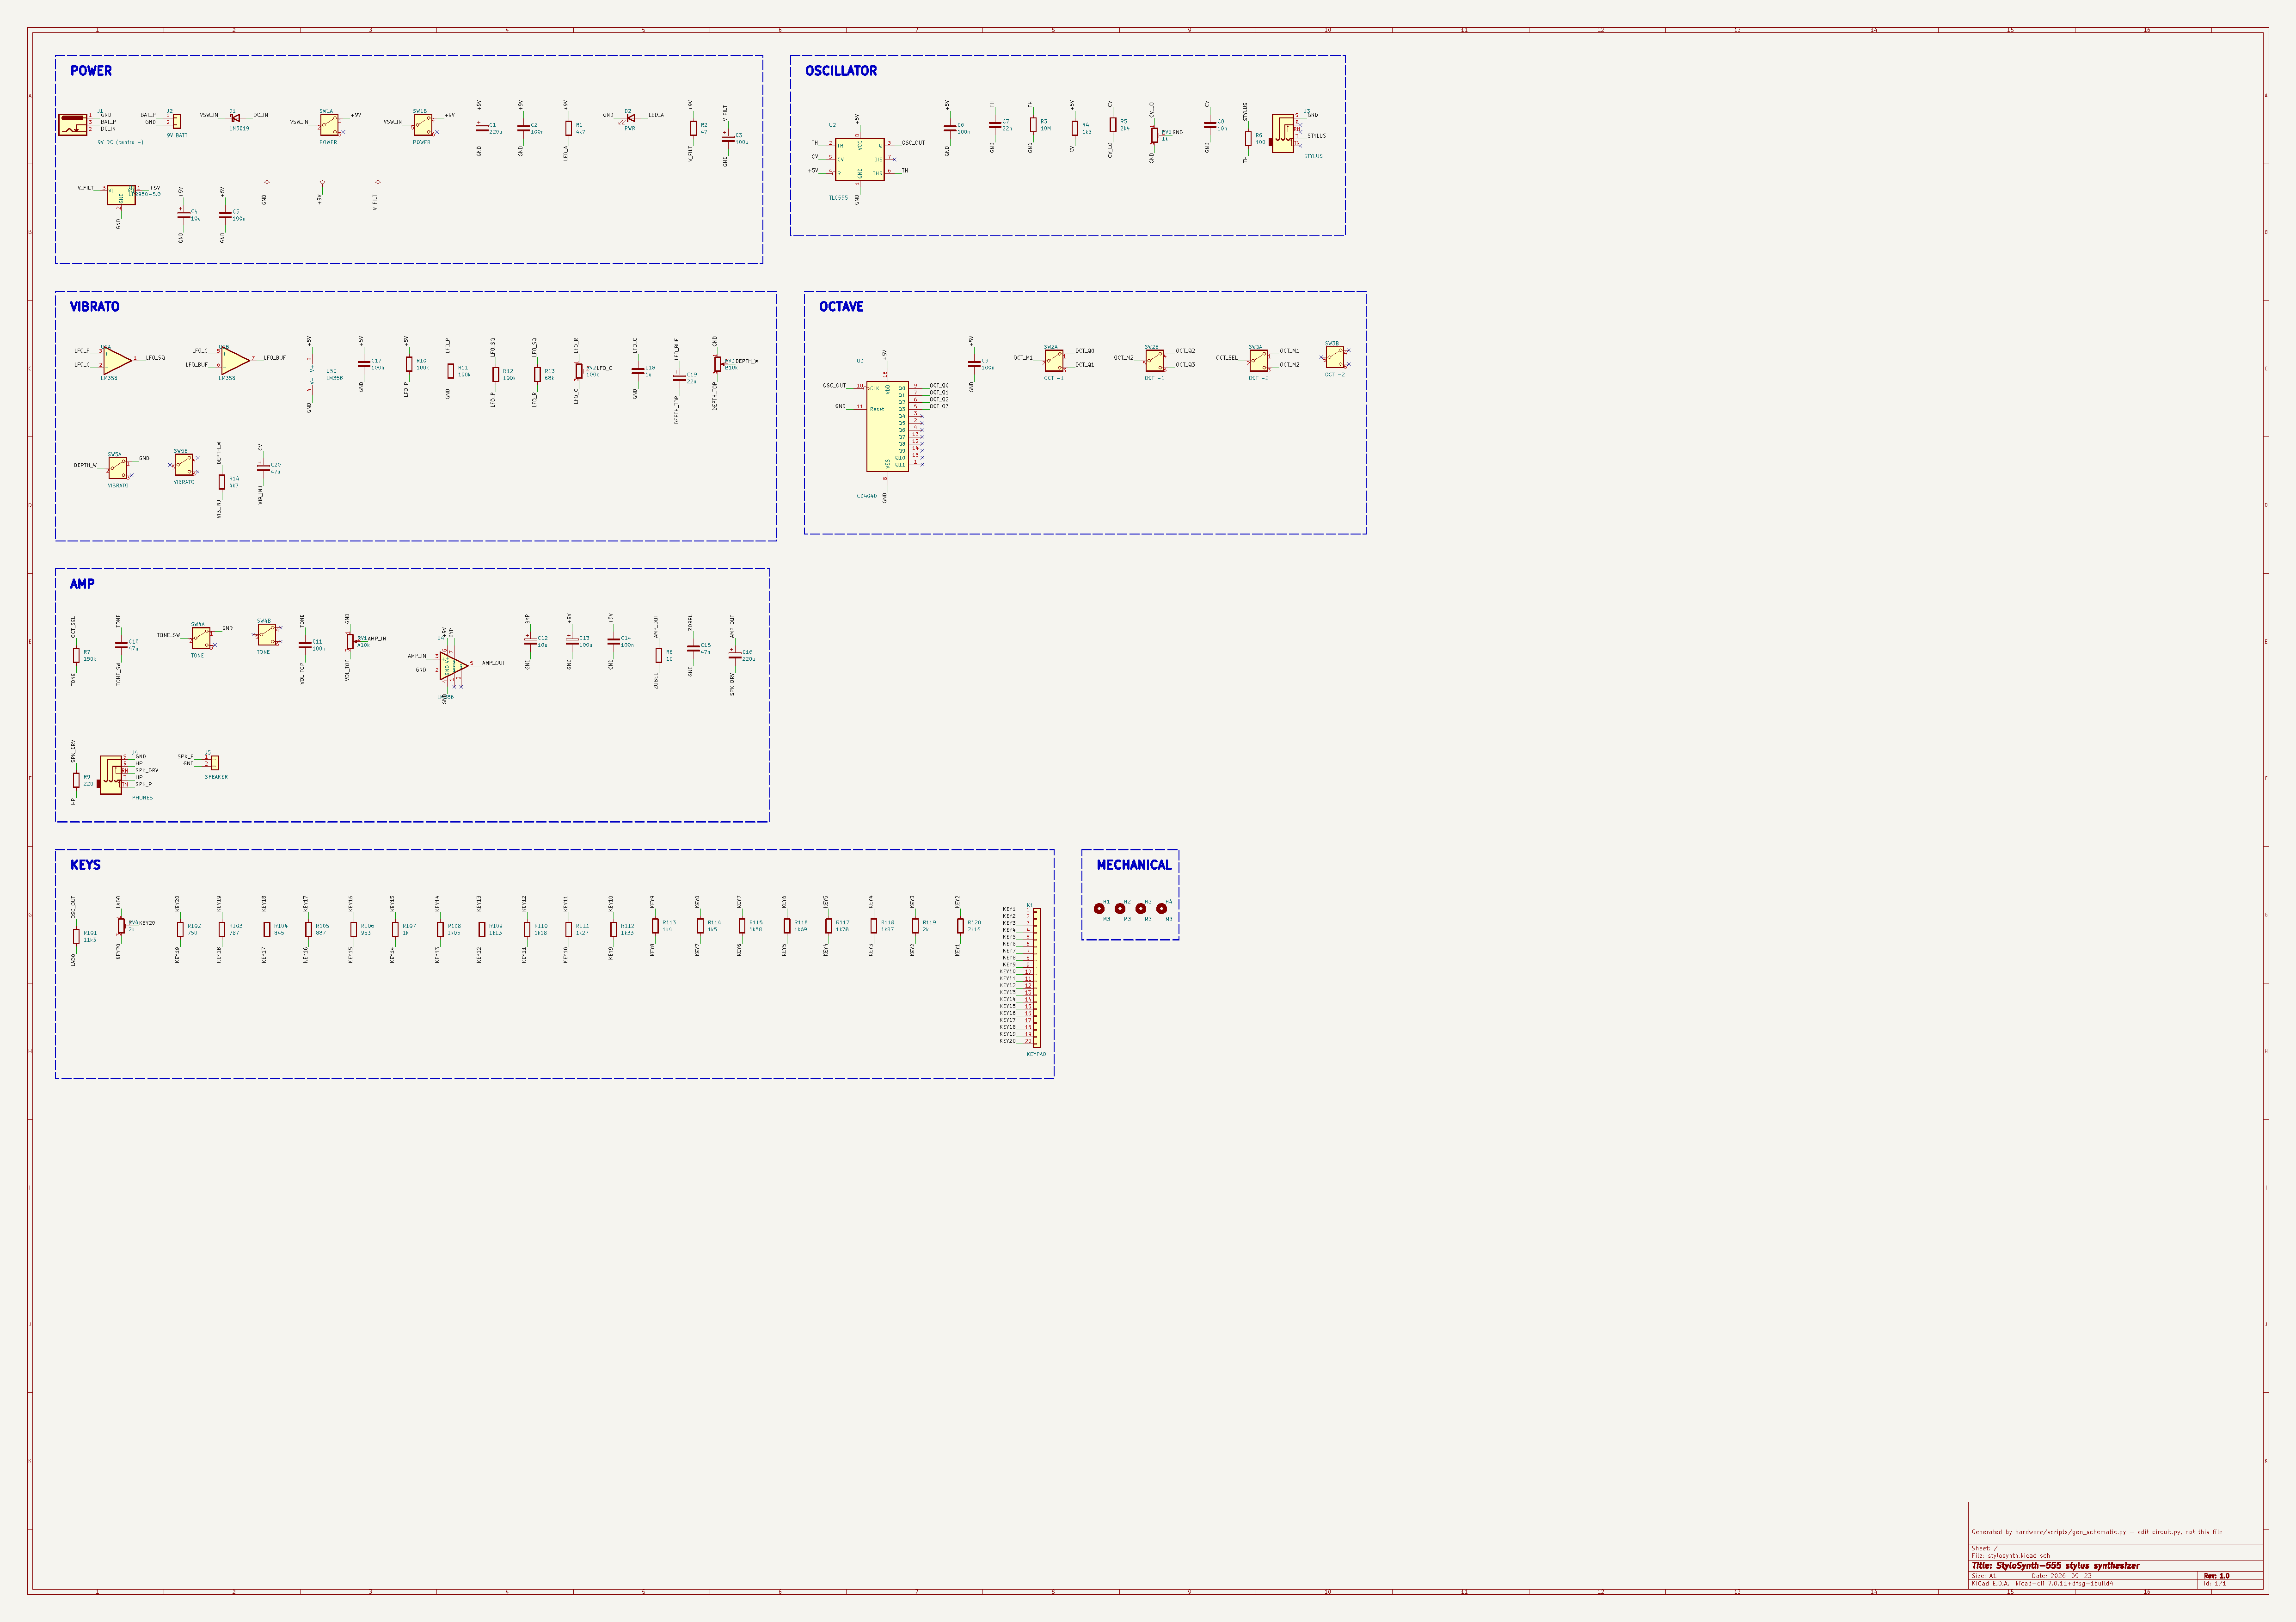
\includegraphics[angle=90, height=0.96\textheight, width=\textwidth, keepaspectratio]{figures/schematic}
\end{center}\restoregeometry
\end{document}